\documentclass[
10pt, % Main document font size
a4paper, % Paper type, use 'letterpaper' for US Letter paper
oneside, % One page layout (no page indentation)
%twoside, % Two page layout (page indentation for binding and different headers)
headinclude,footinclude, % Extra spacing for the header and footer
BCOR5mm, % Binding correction
]{scrartcl}

\usepackage{graphicx}
\usepackage{tikz-er2}
\usepackage[colorlinks, urlcolor=blue, linkcolor=black]{hyperref}

\title{Tp Sistema de Logistica}
\author{Matias M. Marceca}
\date{}

\begin{document}

\maketitle

\tableofcontents

\pagebreak

\section{Idea y Oportunidad de Negocio}

La idea tiene de innovacion la creacion de un sistema modular.
con la posibilidad de sincronizar tareas entre distintas areas
tales como ( proveedores - transportistas - clientes - distribuidoras )
todo por medio de una aplicacion mobile ( Programa ejecutado en un telefono
celular ) sincronizada con servidores en la nube ( Maquinas fisicas accedidas
por medio de Internet ).
\newline\newline
Las necesidades a satisfacer se pueden ver involucradas en una  mayor
organizacion a la hora de gestionar envios de mercaderias desde la salida
del Deposito hasta la puerta del comprador/es,  mejor trazabilidad de
rutas a destinos con verificacion de entregas por medio de consultas a una
base de datos y notificaciones utilizando una aplicacion mobile desde el
punto de entrega del transportista.
\newline\newline
Los beneficios a tener en cuenta son mayor tiempo de busqueda en nuevas
oportunidades de expander el negocio, buscando nuevos clientes para satisfacer
sus necesidades y transportar sus productos, con el soporte y confianza demostrado
teniendo en cuenta la trazabilidad y reportes historicos de clientes sumados
a los casos de exito.
\newline\newline
Al mismo tiempo, otorga tranquilidad y visibilidad en cada etapa del
proceso de entrega de productos, se utiliza un sistema de valoracion de
entregas por medio de la utilizacion de aplicacion una mobile desde el
punto de entrega del cliente para valorar el servicio otorgado por la empresa.
\newline\newline
El cliente compraria nuestro producto porque provee muchas variedades de
soluciones para distintas areas del proceso de transporte de mercaderias cons
una alta confiabilidad y seguridad de datos, con la posibilidad de activar
procesos de guardado de informacion automaticos programables por el usuario
con mayor rango en el sistema. Esta capacidad aumenta que los registros
de los clientes puedan ser guardados en formato portable y generar copias de
seguridad en caso de fallas del ordenador por mal funcionamiento del
sistema operativo.
\newline\newline
Definitivamente este negocio puede generar dinero, la estrategia de venta
va a ser basada en distintos Packs de soluciones por medio de modulos
a demanda del/los cliente/s . Todas las nuevas caracteristicas que el cliente
quiera agregar al producto base no perjudicara el trabajo actual ya realizado
por el cliente, ya que el sistema contara con un administrador de
Plugins ( funcionalidades adicionales que proporcionan mayor versatilidad a un
sistema ya desarrollado ).
\newline\newline
Tambien la empresa contara con contratos diferenciados en tipos de paquetes de
rangos de periodos de tiempo para ofrecer Soporte en horarios de trabajo.

\section {Analsis del Mercado Consumidor}
\subsection {Perfil y Comportamiento del consumidor}
  El surgimiento de la necesidad de logistica para el transporte de
  productos o individuos, se origino en la Ingenieria Militar.
  El objetivo fue trasladar Miles de soldados al mismo tiempo utilizando
  varios y variados metodos evitando que el enemigo note su transporte
  y llegada al objetivo.
  Para llevar a cabo tal plan, se originan los planes de transportes.
  \newline\newline
  Actualmente las Empresas de Logistica tienen como objetivo, planificar el
  traslado de Personas, Productos, Materia Prima, etc, de un lugar a otro.
  Para ello se requiere de una gran infraestructura para poder satisfacer
  varias etapas que cumplen con el objetivo planteado.
  \newline\newline
  Algunas etapas son :
  \begin{itemize}
    \item  Analisis de Trayecto de Mercaderia
    \item  Distribucion de Productos por transporte
    \item  Administracion de Stock de Productos
  \end{itemize}


\subsection {Alcance Estimado}
  Actualmente el Sistema sera de amplio alcance gracias a su facilidad
  de incorporacion y paquetes de modulos en la estrategia de venta, dando
  la posibilidad de obtener la atencion de las medianas y grandes empresas.

\pagebreak
  \textbf {\emph{Listado de Empresas relacionadas a Transporte y Logistica:} }

  \begin{flushleft}
    
\includegraphics[width=17cm, keepaspectratio]{images/list_1.png}
    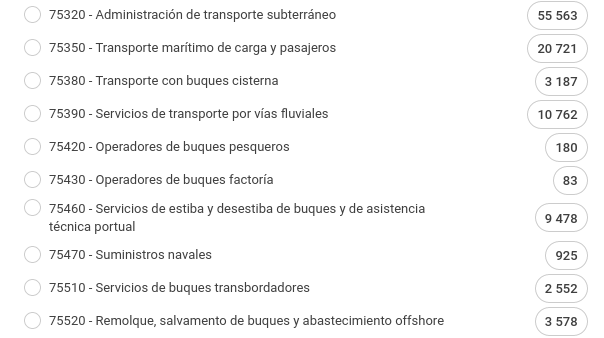
\includegraphics[width=17cm, keepaspectratio]{images/list_2.png}
    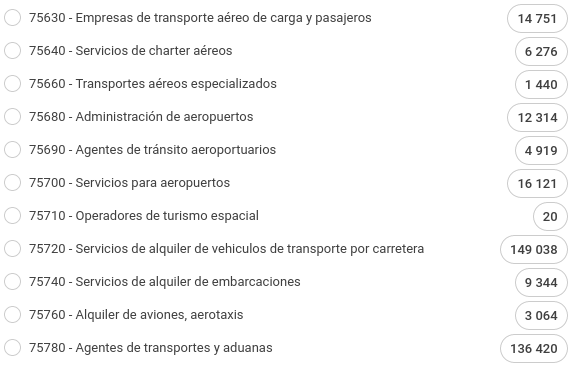
\includegraphics[width=17cm, keepaspectratio]{images/list_3.png}
    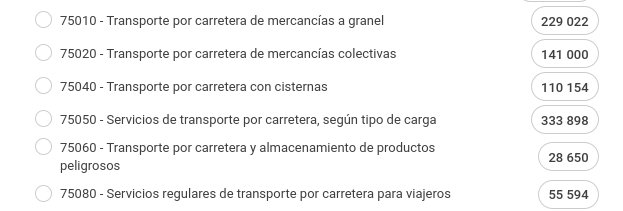
\includegraphics[width=17cm, keepaspectratio]{images/list_4.png}
  \end{flushleft}

\section {Viabilidad de Negocio}

\subsection{Proceso Productivo}
\begin{itemize}
  \item \textbf {Materiales Necesarios}
  \begin{itemize}
    \item Se requiere el uso de \emph { \textbf{6} } discos externos para la
            administracion de guardado de informacion relevante al desarrollo
            del producto.
    \item Se requiere el uso de pendrives para el facil
            y comodo traslado de archivos de video, librerias y graficos
            para ser utilizados el dia que se requiera una presentacion al
            cliente en las oficinas del mismo.
    \item Se requiere utilizar un ambiente de oficina  contando con no mas
            de 20 Grados Cent para una mayor refrigeracion y rendimiento de los
            equipos tecnicos utilizados para lleva a cabo las tareas de desarrollo.
  \end{itemize}

  \item \textbf {Tecnologia Necesaria}
  \begin{itemize}
    \item Se requiere una conexion a Internet, con velocidades no menores a
            1GB de bajada y 500MB de subida para mantener comunicacion
            constante, rapida, confiable e ininterrumpida entre diferentes
            miembros de la empresa. Esto habilita estar a la vanguardia de las
            ultimas actualizaciones en desarrollo y la utilizacion de
            herramientas en Internet para una mayor administracion de los
            procesos de tareas y estado de los desarrollos.
    \item Se requiere la utilizacion de telefonia celular entre los integrantes
            de los equipos para mantener contacto en posibles escenarios donde
            se deba realizar operaciones de soporte fuera de los horarios de
            oficina para el mantenimiento en servidores donde se encuentran
            alojadas los desarrollos realizados y estado de pruebas.

    \item Se requiere de un buen servicio de luz, ya que sin el nada seria
            posible. Como estrategia en caso de emergencias ( un corte de luz ),
            se utilizaria un generador electrico para suministrar los
            equipos electronicos, ya que varios de ellos requieren mantenerse
            prendidos en todo momento.
  \end{itemize}

  \item \textbf {Mano de Obra}
  \begin{itemize}
    \item Para la creacion de la empresa, se requiere de personal capacitado y
            competente acorde a los actuales estandares del desarrollo de sistemas
            de computacion para tener que evitar una previa capacitacion.
  \end{itemize}


  \item \textbf {Insumos}
  \begin{itemize}
    \item Se requiere de \emph { \textbf{33} } monitores de alta gama,
            ya que con ellos, los programadores pueden tener mas herramientas
            a la vista y agilizar su desarrollo tanto como su desempeño a la
            hora de analizar nuevos requerimientos y llevar a cabo las tareas
            necesarias de investigacion, desarrollo y pruebas del producto.
    \item Se requiere de \emph { \textbf{17} } teclados ergonomicos
            ya que los teclados comunes conducen a una postura poco saludable
            para todo aquel que pase mucho tiempo frente a una computadora.
            El desarrollador es la materia prima de la empresa y el teclado
            es su principal herramienta para el ingreso de sus ideas.
    \item Se requiere de \emph { \textbf{17} } mouse (punteros de ordenaror)
            ya que algunas aplicaciones, ya sean utilizadas en internet o de
            escritorio, requieren la accion de presionar sobre botones en la
            pantalla.
\pagebreak

      \item Se requiere de \emph { \textbf{17} } Gabinetes (Caja rectangular
              donde se unen componentes alimentados por cables de electricidad
              unidos a una placa madre que ejecutan las tareas internas del
              ordenador) armados con hardware (Componentes individuales del
              ordenador) capaz de procesar tareas complejas a una velocidad
              rapida y eficiente.
    \item Se requiere de \emph { \textbf{17} } cables de red ya que sin ellos
            los equipos y servidores que requieran de una conectividad
            fluida entre ellos y a Internet, dependerian de una conexion por
            red inalambrica, inestable y mucho mas lenta.
    \item Se requiere de \emph { \textbf{5} } modems ( Dispositivo
            que facilita la conexion entre un ordenador e Internet ) o
            Routers ( Dispositivo que facilita la conexion entre un
            ordenador e Internet u otros dispositivos conectados al mismo
            Router ) Wifi ( Tecnologia de transmision de datos por medio de
            señales de ondas de radio en distintas frecuencias ) para
            conectividad de red sin cable.
    \item Se requiere de \emph { \textbf{1} } expansor de señal Wifi
            para un mayor abastecimiento de señal en todo el edificio y
            no depender de varios Routers para que la señal sea accesible en
            todas las oficinas.
  \end{itemize}
\end{itemize}

\subsection{Localizacion}
\begin{itemize}
  \item \textbf {Comunicaciones}
  \begin{itemize}
    \item Todo tipo de comunicacion se realizaria a traves de Internet en caso
            de que el personal de la empresa se encuentre trabajando desde su
            domicilio (Modalidad Home Office).
  \end{itemize}
\end{itemize}


\subsection{Requerimientos Tecnicos}
\begin{itemize}
  \item \textbf {Tecnologias}
  \begin{itemize}
    \item Librerias de libre uso y distribucion para el manejo de ventanas
          y herramientas varias (Botones ejecutables - Barras de desplazamiento )
          en el sistema operativo objetivo.
  \end{itemize}

  \item \textbf {Estructura Organizacional}
  \begin{itemize}
    \item Lider de Proyecto.
            El lider de proyecto se encarga de asignar las tareas del
            Sprint (Modalidad de desarrollo de entregables al cliente en un
                     tiempo acordado con el cliente no mas de 3 semanas. )
            a cada desarrollador a su cargo y otorgar soporte a los mismos
            en caso de que alguna tarea asignada se haya subestimado y sea
            mas compleja que lo que se estimo desde un principio.
    \item Administrador de Proyecto.
            El administrador de proyecto esta a cargo de administrar las
            prioridades de las tareas que se van a seleccionar por Sprint.
            Los mismos tienen contacto directo con los clientes y deciden
            que tareas son mas importantes que otras dependendiendo de su
            complejidad y etapa del desarrollo.
    \item Desarrolladores
            Los desarrolladores son los encargados de analizar, estimar,
            producir, probar y documentar cada tarea que se le es asignada.
            Tambien tienen la obligacion de avisar a su superior ante cualquier
            contra tiempo por incumplimiento de la fecha de entrega de alguna tarea.
  \end{itemize}
\end{itemize}

\section{Procesos}

\subsection{Mapa de Procesos}
    % this include the content of process_map_content.tex
    %\thispagestyle{empty}

\usetikzlibrary{positioning}
\usetikzlibrary{shadows}

\tikzstyle{strategic} = [top color=white, bottom color=blue!80,
                            draw=yellow!50!black!100, drop shadow]

\tikzstyle{operative} = [top color=white, bottom color=red!80,
                            draw=yellow!50!black!100, drop shadow]

\tikzstyle{support} = [top color=white, bottom color=orange!80,
                            draw=yellow!50!black!100, drop shadow]

\tikzstyle{title} = [top color=white, bottom color=purple!80,
                            draw=yellow!50!black!100, drop shadow]

\centering
\scalebox{.87}{
\begin{tikzpicture}[node distance=1.5cm, every edge/.style={link}]

% Titles
  \node[title]  (estr)                     {Estrategias};
  \node[title]  (oper) [right=4cm of estr] {Operativos};
  \node[title]  (supp) [right=4cm of oper] {Soporte};

% Strategic
  \node[strategic]  (node1) [below=of estr]  {Marketing};
  \node[strategic]  (node2) [below=of node1] {Publicidad};
  \node[strategic]  (node3) [below=of node2] {Contratacion de Personal};
  \node[strategic]  (node4) [below=of node3] {Politicas Financieras};

% Operative
  \node[operative]  (node5) [below=of oper]  {Distribucion de Tareas};
  \node[operative]  (node6) [below=of node5] {Estimacion de Tiempos};
  \node[operative]  (node7) [below=of node6] {Desarrollo del Producto};
  \node[operative]  (node8) [below=of node7] {Pruebas Unitarias};

% Support
  \node[support]    (node9)  [below=of supp]  {Relevacion de Informacion};
  \node[support]    (node10) [below=of node9]  {Planeamiento};
  \node[support]    (node11) [below=of node10] {Pruebas en Servidores};
  \node[support]    (node12) [below=of node11] {Puesta en Produccion};

  % Relations
  \draw[red, thick, dashed] (0,0) (node1)  -- (node2)  ;
  \draw[red, thick, dashed] (node2)  -- (node3)  ;
  \draw[red, thick, dashed] (node3)  -- (node4)  ;

  \draw[red, thick, dashed] (node5)  -- (node6)  ;
  \draw[red, thick, dashed] (node6)  -- (node7)  ;
  \draw[red, thick, dashed] (node7)  -- (node8)  ;

  \draw[red, thick, dashed] (node9)  -- (node10) ;
  \draw[red, thick, dashed] (node10) -- (node11) ;
  \draw[red, thick, dashed] (node11) -- (node12) ;

  \end{tikzpicture}
}



    \thispagestyle{empty}

\usetikzlibrary{positioning}
\usetikzlibrary{shadows}

\tikzstyle{strategic} = [top color=white, bottom color=blue!80,
                            draw=yellow!50!black!100, drop shadow]

\tikzstyle{operative} = [top color=white, bottom color=red!80,
                            draw=yellow!50!black!100, drop shadow]

\tikzstyle{support} = [top color=white, bottom color=orange!80,
                            draw=yellow!50!black!100, drop shadow]

\tikzstyle{title} = [top color=white, bottom color=purple!80,
                            draw=yellow!50!black!100, drop shadow]

\centering
\scalebox{.87}{
\begin{tikzpicture}[node distance=1.5cm, every edge/.style={link}]

% Titles
  \node[title]  (estr)                     {Estrategias};
  \node[title]  (oper) [right=4cm of estr] {Operativos};
  \node[title]  (supp) [right=4cm of oper] {Soporte};

% Strategic
  \node[strategic]  (node1) [below=of estr]  {Marketing};
  \node[strategic]  (node2) [below=of node1] {Publicidad};
  \node[strategic]  (node3) [below=of node2] {Contratacion de Personal};
  \node[strategic]  (node4) [below=of node3] {Politicas Financieras};

% Operative
  \node[operative]  (node5) [below=of oper]  {Distribucion de Tareas};
  \node[operative]  (node6) [below=of node5] {Estimacion de Tiempos};
  \node[operative]  (node7) [below=of node6] {Desarrollo del Producto};
  \node[operative]  (node8) [below=of node7] {Pruebas Unitarias};

% Support
  \node[support]    (node9)  [below=of supp]  {Relevacion de Informacion};
  \node[support]    (node10) [below=of node9]  {Planeamiento};
  \node[support]    (node11) [below=of node10] {Pruebas en Servidores};
  \node[support]    (node12) [below=of node11] {Puesta en Produccion};

  % Relations
  \draw[red, thick, dashed] (0,0) (node1)  -- (node2)  ;
  \draw[red, thick, dashed] (node2)  -- (node3)  ;
  \draw[red, thick, dashed] (node3)  -- (node4)  ;

  \draw[red, thick, dashed] (node5)  -- (node6)  ;
  \draw[red, thick, dashed] (node6)  -- (node7)  ;
  \draw[red, thick, dashed] (node7)  -- (node8)  ;

  \draw[red, thick, dashed] (node9)  -- (node10) ;
  \draw[red, thick, dashed] (node10) -- (node11) ;
  \draw[red, thick, dashed] (node11) -- (node12) ;

  \end{tikzpicture}
}




  \begin{flushleft}
  \textbf{ \emph{Marketing : } } El proceso de \textit{Marketing} estara
  a cargo de la creacion del modelo de negocio para poder generar las ventas.
   \newline \newline
  \textbf{ \emph{Publicidad : } } El proceso de \textit{Publicidad} estara
  a cargo de la imagen, estetica y estrategia artistica para llamar la atencion
  de los consumidores y generar consultas sobre nuestro producto.
   \newline \newline
  \textbf{ \emph{Gestion de Personal : } } La \textit{Gestion de Personal}
  se hara cargo de la administracion de los empleados. En el mismo se debe
  administrar los pagos de cada empleado de la empresa como realizar la busqueda
  de nuevos talentos para la compania cuando sea requerido.
   \newline \newline
  \textbf{ \emph{Gestion de Finanzas : } } La \textit{Gestion  de Finanzas} se
   hara cargo de la administracion de la recaudacion de ingresos monetarios
   adquiridos por parte de contratos establecidos a clientes. A su vez
   estara a cargo de autorizar la incorporacion de nuevos integrantes a la
   empresa como tambien nuevos insumos para mejorar la productividad e
   imagen de la empresa.
   \newline \newline
  \textbf{ \emph{Distribucion de Tareas : } } En la \textit{Distribucion de Tareas}
  se evaluan las prioridades a tener en cuenta para un periodo de dos semanas.
  Estas prioridades son creadas en conjunto entre el cliente y un representante
  tecnico de la empresa ( por lo general un analista funcional ) y se decide
  que nuevas caracteristicas incluir en las siguientes semanas del desarrollo..
  \newline  \newline
  \textbf{ \emph{Estimacion de Tiempos : } } En la \textit{Estimacion de Tiempos}
  se evalua un promedio de tiempo de desarrollo  para las tareas seleccionadas
  en la etapa de \textit{Distribucion de Tareas}. La estimacion promedio de
  cada  tarea a realizar por los desarrolladores la realiza el
  \textit{Lider Tecnico} del equipo en consenso con el \textit{Desarrollador}
  a quien se le asignara la tarea.
  \newline  \newline
  \textbf{ \emph{Desarrollo del Producto : } } En el \textit{Desarrollo del Producto}
  se realizan las tareas asignadas en el proceso de \textit{Distribucion de Tareas}.
  Las mismas son esperadas que se realicen en el tiempo establecido y acordado
  entre el \textit{Desarrollador} y el \textit{Lider Tecnico}.
  \newline  \newline
  \textbf{ \emph{Pruebas de Integracion : } } En el proceso de
  \textit{Pruebas de Integracion} se realizan pruebas \emph{Funcionales} de
  las distintas caracteristicas del producto. Por Ejemplo,
  \newline
  \& "\textsc{Entrada de Clientes}", "\textsc{Exportacion de Datos}".
  \newline  \newline
  \textbf{ \emph{Relevamiento de Informacion : } } En el proceso de
  \textit{Relevamiento de Informacion} se realiza una reunion con el cliente
  para generar nuevos comportamientos y funcionalidades que pueden llevar al
  sistema a su siguiente nivel. En dicha reunion deben obtenerse que necesidades
  no estan integradas actualmente en el sistema y son requeridas por el cliente.
  Para ello se debe obtener informacion de como son los procesos actuales del
  cliente para comprender mejor sus espectativas y brindar soluciones que
  asceleren su productividad.
  Por Ejemplo,
  "\textsc{Mapa de actuales entregas en proceso}",
  "\textsc{Calendario para seguimiento de entregas}",
  "\textsc{Envio automatico de notificaciones a clientes sobre el estado del envio}".
  \newline  \newline
  \textbf{ \emph{Planeamiento : } } En el proceso de \textit{Planeamiento} se
  distribuyen las nuevas funcionalidades generales de cada area del sistema y
  son entregadas a cada \textit{Lider Tecnico} para empezar con el proceso de
  \textit{Distribucion de Tareas}.
  \newline  \newline
  \textbf{ \emph{Pruebas en Servidores : } } El proceso de
  \textit{Pruebas en Servidores} se realiza una instalacion de ambiente
  de prueba de todo el sistema. La particularidad de este proceso es que
  se realiza en servidores del cliente y es un simulacro de utilidad del mismo.
  Se instala el sistema ya desarrollado para que personal del cliente lo
  utilice como si estviera en un entorno productivo. Los beneficion que esta
  trae, es que pueden encontrar errores que el \textit{Desarrollador} no tuvo
  en cuenta.
  \newline  \newline
  \textbf{ \emph{Puesta en Produccion : } } En el proceso de
  \textit{Puesta en Produccion} se realiza la instalacion del ambiente
  definitivo del sistema. Se realiza en horarios donde los operarios del mismo
  tienen la menor carga operacional para que la transicion de datos pueda
  realizarse de manera correcta y con menor riesgo de perdida de informacion.
  Se acuerda un periodo de tiempo para llevar a cabo el proceso y puede
  finalizar en un resultado \textsc{Positivo} o \textsc{Negativo} teniendo
  que corregir los errores dados en el proceso y acordar una nueva fecha de
  instalacion del sistema.
  \end{flushleft}

\section{Referencias}

\begin{itemize}
  \item \textit{Origen de la Logistica :} \href{https://clusterlogistic.org/es/historia-de-la-logistica/} {Link}
  \item \textit{Listado de Empresas seleccionadas:} \href{https://ar.kompass.com/buy-company-list/} {Link}
\end{itemize}

\end{document}


% Just in case of need
% std nus: ( normal computer user )
%   tec : 1
%   mou : 1
%   cpu : 1
%   aur : 1
%   caR : 1 (cable de red rj45)

% std hr:   ( human resource )
%   nus : 1
%   mon : 1
%

% std dev / tl / des:  ( Software Developer / team leader / designer )
%   use : 1
%   mon : 2
%
% dev / des team:
%   dev: 3
%    tl: 1
%   dex: 1  ( discos externos )
%   pen: 2  ( pendrives )
%   rou: 1  ( router )
%
% Prd Area:
%   dvt: 3  ( Dev team )
%   dst: 1  ( Des team )

% Spa Area:     ( Spare Time Area )
%   exs : 1  ( Wife signal Expansor )

% building:
%    par: 1  ( prodction area on building )
%    sar: 1  ( spare time area  on building )
